\documentclass[tikz,border=2pt]{standalone}
\usepackage{amsmath,amssymb}
\usepackage{pgfplots}
\pgfplotsset{compat=1.18}
\usetikzlibrary{calc}

\begin{document}
% Along any segment from x to y the graph of a convex function lies below the chord, that
% of a concave function above it; on R^n the same test is applied to every segment.
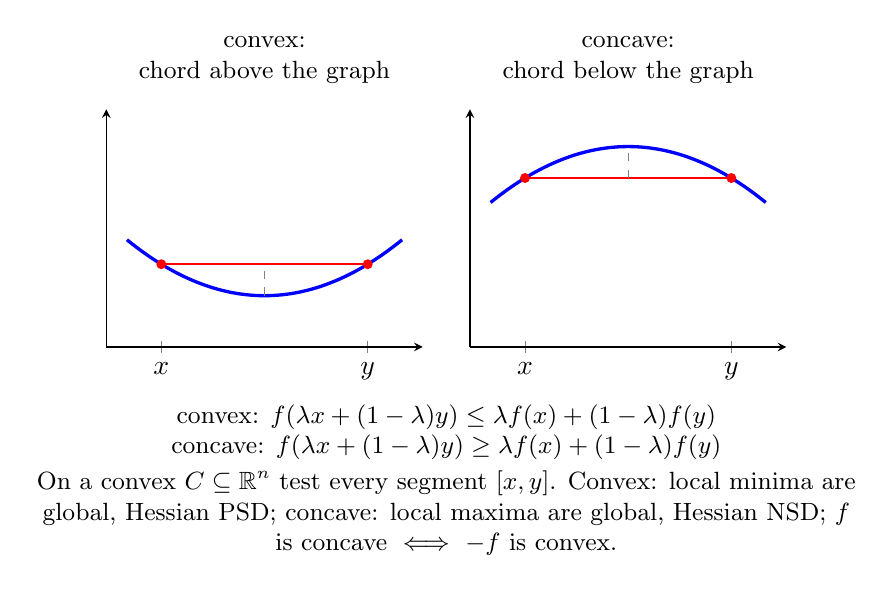
\begin{tikzpicture}
	\begin{axis}[
		name=p1, axis lines=left, xmin=-0.3, xmax=4.3, ymin=-0.3, ymax=4.8,
		xtick={0.5,3.5}, xticklabels={$x$,$y$}, ytick=\empty,
		samples=80, smooth, width=5.6cm, height=4.6cm, clip=false, title={convex:\\ chord above the graph}, title style={font=\small, align=center}
		]
		\addplot[blue, very thick, domain=0:4] {0.3*(x-2)^2+0.8};
		\draw[red, thick] (axis cs:0.5,1.475) -- (axis cs:3.5,1.475);
		\fill[red] (axis cs:0.5,1.475) circle (1.8pt);
		\fill[red] (axis cs:3.5,1.475) circle (1.8pt);
		\draw[gray, dashed] (axis cs:2,0.8) -- (axis cs:2,1.475);
			\end{axis}
	\begin{axis}[
		name=p2, at={(p1.east)}, anchor=west, xshift=0.6cm,
		axis lines=left, xmin=-0.3, xmax=4.3, ymin=-0.3, ymax=4.8,
		xtick={0.5,3.5}, xticklabels={$x$,$y$}, ytick=\empty,
		samples=80, smooth, width=5.6cm, height=4.6cm, clip=false, title={concave:\\ chord below the graph}, title style={font=\small, align=center}
		]
		\addplot[blue, very thick, domain=0:4] {4-0.3*(x-2)^2};
		\draw[red, thick] (axis cs:0.5,3.325) -- (axis cs:3.5,3.325);
		\fill[red] (axis cs:0.5,3.325) circle (1.8pt);
		\fill[red] (axis cs:3.5,3.325) circle (1.8pt);
		\draw[gray, dashed] (axis cs:2,3.325) -- (axis cs:2,4);
			\end{axis}
	\path (p1.outer south west) -- (p2.outer south east) node[midway, anchor=north, align=flush center, text width=10.4cm, font=\small, yshift=-2pt] {convex: $f(\lambda x+(1-\lambda)y)\le\lambda f(x)+(1-\lambda)f(y)$\\ concave: $f(\lambda x+(1-\lambda)y)\ge\lambda f(x)+(1-\lambda)f(y)$\\[2pt] On a convex $C\subseteq\mathbb{R}^n$ test every segment $[x,y]$. Convex: local minima are global, Hessian PSD; concave: local maxima are global, Hessian NSD; $f$ is concave $\iff$ $-f$ is convex.};
\end{tikzpicture}
\end{document}
